\documentclass[11pt,runningheads,a4paper]{article}
\usepackage[utf8]{inputenc}
\usepackage{amsmath,amssymb,hyperref,array,xcolor,multicol,verbatim,mathpazo,float}
\usepackage[normalem]{ulem}
\usepackage[pdftex]{graphicx}
\usepackage{fullpage}
\usepackage{hyperref}
\usepackage{float}
\usepackage{listings} % code highlighting
\newcommand{\DNA}[1]{\texttt{\uppercase{#1}}}
\begin{document}
% notes to resolve sometimes:
% hierarchical O(n^2) wrong
% crooked casino example wrong
% Formulas V-learning, BaumWelch (transition emissions not in slides)

\title{{\LARGE Bioinformatics Supervision}\\
{\Large Michaelmas Term 2017}\\
{\Large --Problem Sheet 3--}} 

\author{Supervisor: Sebastian Müller (Department of Plant Sciences)}
\date{}

\maketitle

Please hand in your work 24 hours prior to the supervision either to \texttt{sm934@cam.ac.uk} or at the Plant Sciences Department reception (make sure my name is on it). 
Feel free to team up with other group members, the main aim is to understand the material. 
If you hand in electronically, please name the file \texttt{group<x>\_<crsid>\_problemsheet<x>.<x>}

\begin{enumerate}

\section*{Hidden Markov Models}
\label{sec:hidden_markov_models}

  \item Consider the following Hidden Markov Model. In this approximation, H represents DNA coding segments (high GC content), whereas L represents DNA non-coding segments (low GC content).
    \begin{figure}[H]
      \centering
      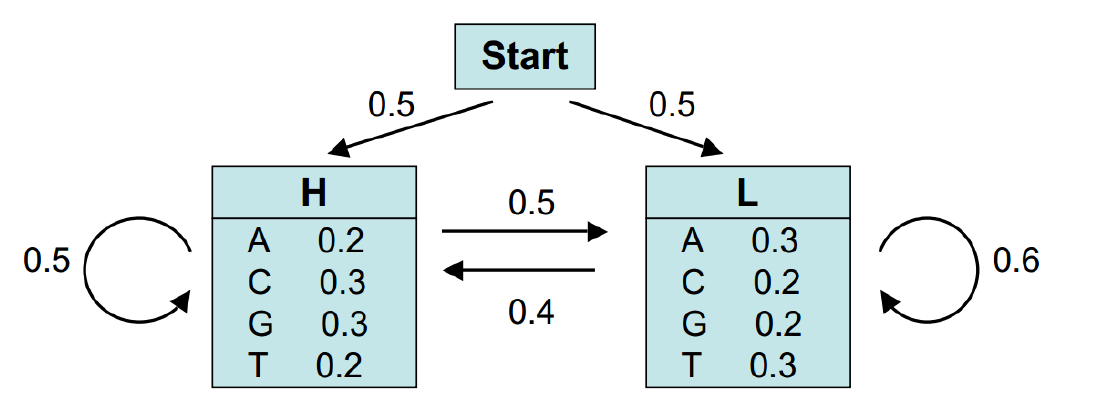
\includegraphics[scale=0.35]{img/Bioinformatics_Problem_Sheet3_Figure1.png}
    \end{figure}
  \begin{enumerate}
  \item Use Forward Algorithm to find the probability sequence GGCA was generated by this model.
% what about "+" step
  \item Use the Viterbi Algorithm to determine the most probable path through the model for the sequence GGCACTGAA (hint: you could also use log-probabilities).
  \end{enumerate}
  \item Describe how you would build a hidden Markov model (HMM) to identify membrane segments in amino-acid sequences\@. 
    How you would assess the sensitivity and specificity of your HMM?
  \item Describe briefly Viterbi learning and Baum-Welch learning. What is the main difference?
    
\section*{Genome assembly}
\label{sec:genome_assembly}


  \item For de Brujin graphs, why are we assigning the k-mers of a string to edges instead of the nodes?
  \item Given the following string s = \DNA{ATTACGGTACCCCTACA}
    \begin{enumerate}
      \item \label{item:a} Construct the de Brujin graph with $k=3$ for string $s$.
      \item \label{item:b} Construct a paired de Brujin graphs with $k=3$ and distance $d=1$ for string $s$.
      \item Find all eulerian paths for the graphs in \ref{item:a} and \ref{item:b}\@. What do you notice?
      \item Find all contigs for the graphs in \ref{item:a} and \ref{item:b}\@. What do you notice?
    \end{enumerate}

\section*{Clustering}
\label{sec:clustering}

\item  Explain the two high-level steps taken by the expectation-maximisation (EM) algorithm, and then show how it relates to soft k-means clustering (giving particular care to the stiffness parameter).
  \item  What is the output of a typical gene expression experiment, and why might one wish to do further processing on such a result?
  \item Discuss the properties of the Markov clustering algorithm and the differences with respect to the k-means and hierarchical clustering algorithms.
  \item How can you evaluate the results obtained? 
Describe one external as well as internal validity index of your choice (this paper might get you started: \url{http://www.universitypress.org.uk/journals/cc/20-463.pdf}). 
What do you think are their limitations?
% good cluster principle
    %\item Try out Markov clustering at the BiGRe laboratory (\url{http://rsat.scmbb.ulb.ac.be/index_neat.html}).  Click on ‘MCL Clustering’, under ‘Clusters/Networks’ (on the left of the screen), then on ‘DEMO’.
    %\begin{enumerate}
    %\item Can you explain the demonstration dataset?
    %\item Click ‘GO’ to start the clustering process. Describe the graph produced as a result.
    %\item Save the clusters (tab format) and submit them along with your answers
    %\item Map the clusters by clicking on ‘Map those clusters on the network’, then ‘GO’. View the clusters by clicking on ‘Display the graph’, then ‘GO’. Include a screenshot in your answers.
    %\end{enumerate}

\subsection*{Optional tasks}
Feel free to complete as much as you feel confident.

One of the most popular programming language in bioinformatics is R (\url{https://cran.r-project.org/}).

Try to run and understand the following code:

\lstdefinestyle{customc}{
  belowcaptionskip=1\baselineskip,
  breaklines=true,
  frame=L,
  xleftmargin=\parindent,
  language=S,
  showstringspaces=false,
  basicstyle=\footnotesize\ttfamily,
  %keywordstyle=\bfseries\color{green!40!black},
  commentstyle=\itshape\color{gray},
  %identifierstyle=\color{blue},
  stringstyle=\color{orange},
}

\lstset{language=S,style=customc}
\begin{lstlisting}
head(iris) #inspecting iris dataset
str(iris)  #still inspecting
?help(iris)
dd <- dist(scale(iris[,-5]), method = "euclidean") #creating distance matrix
hc <- hclust(dd, method = "average") #UPGMA clustering
plot(hc)
\end{lstlisting}

\item Familiarise yourself with the iris dataset (see code above) as well as distance matrices \lstinline{(help(dist))}, could you think of any situations the euclidean distance is not appropriate?
\item Familiarise yourself with the hierarchical clustering function (help(hclust)).
\item Familiarise yourself with $cutree$ \lstinline{(help(cutree))}. Whats the point of this function?

\begin{enumerate}
  \item Investigate the 3 cluster solution\lstinline{(table(cutree(hc,3)))}.
\item Compare the 3 cluster solution with the actual classification (stored column 5).

  \lstinline{table(cutree(hc,3), iris[,5])}.
\item How do you interpret this table? Is this result expected?
\item Would it improve if you took the 4 cluster solution instead? How about using the default Ward clustering instead UPGMA?
\end{enumerate}

\item Try to write code to compute the euclidean distances yourself
\item Very optional: try to write code to perform UPGMA clustering yourself and run it on the distance matrix dd.
\end{enumerate}
%% Those have been taken out from Piotres Lecture as of Michalmas Term 2016
%\item Read the lecture notes on Gibbs Sampling for motif detection, then watch the lecture series on
%Youtube on the same topic: https://www.youtube.com/watch?v=KqquwB_kHvU,
%https://www.youtube.com/watch?v=m2NV1ET0ZqY, https://www.youtube.com/watch?v=-
%cuduZSC_ks and https://www.youtube.com/watch?v=JCk0PJL6bCY. Can you write your own
%explanation of the Gibbs Sampling technique that is clearer than the one the lecturer gave you?
%\item What is the difference between the adjacency list and the accessibility list?
%\item Apply the Wagner algorithm to the following accessibility list in order to reconstruct its adjacency
%list and thereby describe the network from which it originated.
%\item In modelling a metabolic process, describe advantages and disadvantages of using a stochastic
%approach (for example agents) as opposed to using a set of deterministic differential equations.
%\item Describe the Gillespie algorithm and discuss its relationship with genetic/biochemical networks
%\item Consider the following model for a simple gene regulation network with only one gene. Apply
%the Gillespie algorithm to determine the probability and order in which each event occurs, along
%with an equation for the time of its occurrence. You will need to include a new random variable for
%each step. Wherever a choice is probability dependent, assume the most likely event occurs first.
%\item Along with the model above, you can find five other biological models to try out here:
%http://mosi.cs.uni-saarland.de/wp-content/uploads/2013/11/Exercise_6.pdf. The exercise suggests
%that you write your own MATLAB code to determine the trajectories for each of these models. This is
%fine if you feel like doing this, but I would suggest that you use a library to do this for you. For
%example, I have found the GillespieSSA package for R to be very easy to use. As an example, below
%you can find the code I have written (using this package) for the model in question 11:
%parms <- c(c1=1, c2=1, c3=4, c4=10)
%x0 <- c(DNA_OFF=1,DNA_ON=0,MRNA=0)
%a <- c("c1*DNA_OFF","c2*DNA_ON","c3*DNA_ON", "c4*MRNA")
%nu <- matrix(c(-1,+1,0,0,+1,-1,-1,0,0,0,+1,-1),nrow=3,byrow=TRUE)
%out <- ssa(x0,a,nu,parms,tf=10,simName="Simple Gene Regulation Network")
%x11()
%plot(x=out$data[,1],out$data[,2],col="red",type="l",xlab="Time",ylab="State
%Value",main=out$args$simName)
%lines(x=out$data[,1],out$data[,3],col="blue")
%lines(x=out$data[,1],out$data[,4],col="green")
%legend("topright",legend=c("DNA_OFF","DNA_ON","MRNA"),lty=1,col=c("red","bl
%ue","green"),bg = "gray90")
%If you would like me to cover something more in the supervision, please let me know in advance

\end{document}
